\subsection{Schroedinger and Heisenberg picture}
\subsubsection{Schroedinger picture}
In the Schroedinger picture, we focus on the time evolution of states:
\begin{equation}  
	|\psi\rangle = |\psi\rangle(t) 
\end{equation}
In this picture we can introduce quantum circuit diagram notation, whereby:
\begin{itemize}
	\item States progress in time along horizontal parallel lines
	\item Time goes from left to right
	\item Gates denoted X,Y,Z are the pauli matrices 
		$\sigma_x,\sigma_y,\sigma_z$
	\item Gates can act on one or multiple qubits, whereby an X gate 
		on qubit 1 in a 3-qubit system should be interpreted as:
		\\$(X\otimes \mathbb{I} \otimes \mathbb{I}) (|\psi_1\rangle
		\otimes |\psi_2\rangle \otimes |\psi_3\rangle)$
\end{itemize}
\begin{figure}[h!]
	\begin{center}
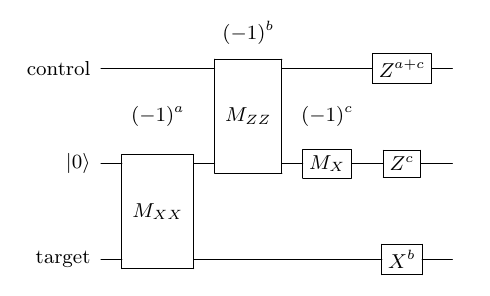
\includegraphics[scale=0.5]{img/cnotMeasureCircuit.png}\\
	\caption{A Quantum Circuit, where $|0\rangle$ is the +1
	eigenstate in $\sigma_z$-basis}
	\label{fig:circuit1}
	\end{center}
\end{figure}
\newpage

In the quantum circuit depicted in figure \ref{fig:circuit1} the input
state can be written as $|\psi_{control}\rangle \otimes |0\rangle 
\otimes |\psi_{target}\rangle$ and the measurement in the first 
timestep can be expressed as $\mathbb{I}\otimes X \otimes X$.\\
To simplify calculation we can write $|\psi_{target}\rangle$ as
$\alpha |0\rangle + \beta |1\rangle$%, where $|+\rangle,|-\rangle$ are
%the +1 and -1 Eigenstates of the $\sigma_x$-matrix. \\
\\
The input state is thus: 
$|\psi_{control}\rangle \otimes |0\rangle 
\otimes( \alpha |0\rangle + \beta |1\rangle)$.\\
The initial state $|\phi_{t=0}\rangle$ = $|\psi_{control}\rangle \otimes |\psi_{ancilla}\rangle \otimes
|\psi_{target}\rangle$\\
where\\
$|\psi_{control}\rangle = \alpha|0\rangle+\beta|1\rangle$
\\
$|\psi_{ancilla}\rangle = |0\rangle$
\\
$|\psi_{target}\rangle = \gamma|0\rangle+\delta|1\rangle$
\\
therefore:
\begin{equation}
|\phi_{t=0}\rangle = \alpha \left( \gamma |000\rangle + \delta |001\rangle\right)+
\beta \left( \gamma |100\rangle + \delta |101\rangle \right)
\end{equation}
If the first measurement result is +1, the state becomes:
\begin{align*}
	|\phi^{+}_{t=1}\rangle 
	&= \frac{1}{2}\left(\mathbb{I}\otimes\mathbb{I}\otimes\mathbb{I}+
	\mathbb{I}\otimes X \otimes X\right)|\phi_{t=0}\rangle\\
	&= \alpha \left( 
	\gamma \left( |000\rangle + |011\rangle \right) +
	\delta \left( |001\rangle + |010\rangle \right) \right) \\
	&+ \beta \left(
	\gamma \left( |100\rangle + |111\rangle \right) +
	\delta \left( |101\rangle + |110\rangle \right) \right)
\end{align*}
if the result is -1, it becomes:
\begin{align*}
	|\phi^{-}_{t=1}\rangle 
	&= \frac{1}{2}\left(\mathbb{I}\otimes\mathbb{I}\otimes\mathbb{I}-
	\mathbb{I}\otimes X \otimes X\right)|\phi_{t=0}\rangle\\
	&= \alpha \left( 
	\gamma \left( |000\rangle - |011\rangle \right) +
	\delta \left( |001\rangle - |010\rangle \right) \right) \\
	&+ \beta \left(
	\gamma \left( |100\rangle - |111\rangle \right) +
	\delta \left( |101\rangle - |110\rangle \right) \right)
\end{align*}

In the case of the +1 Measurement $\rightarrow$ a=0:
\begin{align*}
	|\phi^{++}_{t=2}\rangle 
	&= \frac{1}{2}\left(\mathbb{I}\otimes\mathbb{I}\otimes\mathbb{I}+
	Z\otimes Z \otimes \mathbb{I}\right)|\phi^{+}_{t=1}\rangle\\
	&= (|000\rangle\langle000| +|001\rangle\langle001| +
	|110\rangle\langle110| +|111\rangle\langle111|)|\phi^{+}_{t=1}\rangle\\
	&= \alpha \left( \gamma |000\rangle + \delta |001\rangle \right)
	+ \beta \left( \gamma |111\rangle + \delta |110\rangle\right) 
\end{align*}
\begin{align*}
	|\phi^{+-}_{t=2}\rangle 
	&= \frac{1}{2}\left(\mathbb{I}\otimes\mathbb{I}\otimes\mathbb{I}-
	Z \otimes Z \otimes \mathbb{I}\right)|\phi^{+}_{t=1}\rangle\\
	&= (|010\rangle\langle010| +|011\rangle\langle011| +
	|100\rangle\langle100| +|101\rangle\langle101|)|\phi^{+}_{t=1}\rangle\\
	&= \alpha \left( \gamma |011\rangle + \delta |010\rangle \right)
	+ \beta \left( \gamma |100\rangle + \delta |101\rangle \right) 
\end{align*}
In the case of the -1 Measurement $\rightarrow$ a=1:
\begin{align*}
	|\phi^{-+}_{t=2}\rangle 
	&= \frac{1}{2}\left(\mathbb{I}\otimes\mathbb{I}\otimes\mathbb{I}+
	Z\otimes Z \otimes \mathbb{I}\right)|\phi^{-}_{t=1}\rangle\\
	&= \alpha \left( \gamma |000\rangle + \delta |001\rangle \right)
	- \beta \left( \gamma |111\rangle + \delta |110\rangle\right) 
\end{align*}
\begin{align*}
	|\phi^{--}_{t=2}\rangle 
	&= \frac{1}{2}\left(\mathbb{I}\otimes\mathbb{I}\otimes\mathbb{I}-
	Z\otimes Z \otimes \mathbb{I}\right)|\phi^{-}_{t=1}\rangle\\
	&= - \alpha \left( \gamma |011\rangle + \delta |010\rangle \right)
	+ \beta \left( \gamma |100\rangle + \delta |101\rangle \right) 
\end{align*}
Now the applied measurement is 
$\mathbb{I} \otimes X \otimes \mathbb{I}$, which means:
\begin{align*}
	|\phi^{+++}_{t=3}\rangle 
	&= \frac{1}{2}\left(\mathbb{I}\otimes\mathbb{I}\otimes\mathbb{I}+
	\mathbb{I}\otimes X \otimes \mathbb{I}\right)|\phi^{++}_{t=2}\rangle\\
	&= \frac{1}{2}((|010\rangle + |000\rangle)\langle000|
	+ (|011\rangle + |001\rangle)\langle001|\\
	&+ (|000\rangle + |010\rangle)\langle010|
	+ (|001\rangle + |011\rangle)\langle011|\\
	&+ (|110\rangle + |100\rangle)\langle100|
	+ (|111\rangle + |101\rangle)\langle101|\\
	&+ (|100\rangle + |110\rangle)\langle110|
	+ (|101\rangle + |111\rangle)\langle111|)
	|\phi^{++}_{t=2}\rangle\\
	&= \frac{1}{2}(\alpha \left( 
	\gamma (|000\rangle + |010\rangle)+
	\delta (|011\rangle + |001\rangle) \right) \\
	&+ \beta \left( 
	\gamma (|101\rangle + |111\rangle)+
	\delta (|100\rangle + |110\rangle) \right))
\end{align*}
In this case, a,b and c would each be zero, therefore no further gate would be applied.\\
As intended, this state is equivalent to 
$CNOT_{Control\rightarrow Target} |\phi_{t=0}\rangle$.

